%Master File:lectures.tex


\lesson{Information Theory}
\vspace{-1cm}
\begin{center}
  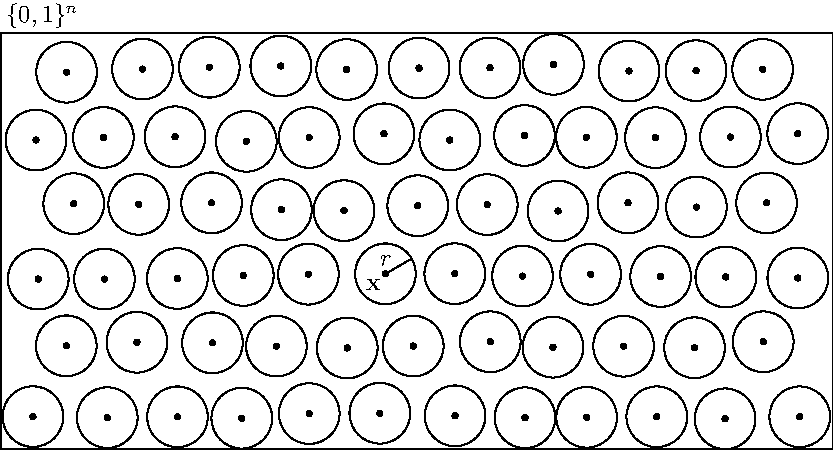
\includegraphics[height=10cm]{shannonBound}
\end{center}
\keywords{Information, KL-divergence, Minimum Description Length}
%%%%%%%%%%%%%%%%%%%%%%% Next Slide %%%%%%%%%%%%%%%%%%%%%%%
\renewcommand{\Outline}{%
\begin{slide}
\section[1]{Outline}

\begin{minipage}{10cm}\raggedright
  \begin{enumerate}\squeeze
    \outlineitem{Information Theory}{info}
    \outlineitem{KL-Divergence}{kldivergence}
    \outlineitem{Minimum Description Length}{mlp}
    \outlineitem{Variational Auto-Encoders}{vae}
  \end{enumerate}
\end{minipage}\hfill
\begin{minipage}{12cm}
  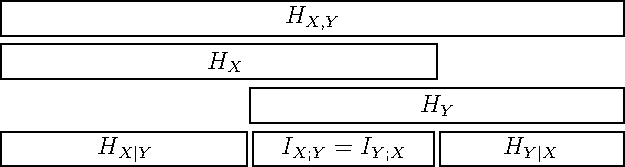
\includegraphics[width=12cm]{mutualinf}
\end{minipage}
\end{slide}
\addtocounter{outlineitem}{1}
}

\newcommand{\bits}{\,\mathrm{bits}}
\setcounter{outlineitem}{1}


%%%%%%%%%%%%%%%%%%%%%%% Next Slide %%%%%%%%%%%%%%%%%%%%%%%
\Outline % Information Theory
%%%%%%%%%%%%%%%%%%%%%%% Next Slide %%%%%%%%%%%%%%%%%%%%%%%


\begin{slide}
\section[-1]{Communicating Via a Noisy Channel}

\begin{PauseHighLight}\small
  \begin{itemize}
  \item Information theory considers communicating down a (noisy)
    channel
    \begin{align*}
      X \sim \Prob{X}  \stackrel{\text{noisy
      channel}}{\xrightarrow{\hspace*{5cm}}} Y \sim \Prob{Y\mid X}
    \end{align*}
  \item  We send a message $X$ (with probability $\Prob{X}$) and
    receive a message $Y$ with probability $\Prob{Y\mid X}$\pause
  \item The uncertainty of the message sent, given we received a
    message $y$ is
    \begin{align*}
      H_{X|Y=y} = - \sum_{x\in\mathcal{X}} \Prob{X=x \mid Y=y} \, \logg{\Prob{X=x \mid Y=y}}\pause
    \end{align*}
  \item The expected uncertainty in the message sent is
    \begin{align*}
      H_{X|Y} = \sum_{y\in\mathcal{Y}} \Prob{Y=y} \, H_{X|Y=y}
      = - \sum_{x,y} \Prob{X=x,Y=y} \, \logg{\Prob{X=x \mid Y=y}}\pause
    \end{align*}
  \end{itemize}
\end{PauseHighLight}

\end{slide}

%%%%%%%%%%%%%%%%%%%%%%% Next Slide %%%%%%%%%%%%%%%%%%%%%%%

\begin{slide}
\section[-1]{Joint Entropy}

\begin{PauseHighLight}
  \begin{itemize}
  \item We can define the \emph{joint entropy}
    \begin{align*}
      H_{X,Y} = - \sum_{x,y} P_{X,Y}(x,y) \logg{P_{X,Y}(x,y)}\pause
    \end{align*}
  \item If the message we receive is independent of the message that
    is sent then $H_{X,Y} = H_X + H_Y$ (we saw this in the last
    lecture)\pause
  \item $H_{X,Y} \neq H_X + H_Y$ if $X$ and $Y$ are correlated\pause
  \item Since $\Prob{X,Y} = \Prob{Y|X}\,\Prob{X} =
    \Prob{X|Y}\,\Prob{Y}$ if follows
    \begin{align*}
      H_{X,Y} = H_{X} + H_{Y|X} = H_{Y} + H_{X|Y}\pause
    \end{align*}
  \item Or $H_{X} - H_{X|Y} = H_{Y} - H_{Y|X}$\pause
  \end{itemize}
\end{PauseHighLight}

\end{slide}


%%%%%%%%%%%%%%%%%%%%%%% Next Slide %%%%%%%%%%%%%%%%%%%%%%%

\begin{slide}
\section{Mutual Information}

\begin{PauseHighLight}
  \begin{itemize}
  \item The amount of uncertainty about the message being sent, $X$,
    before receiving the message is
    $H_X=-\av[X]{\log{\Prob{X}}}$\pause
  \item Shannon define the \textit{mutual information} to be the expected loss
    in uncertainty when we receive a message
    \begin{align*}
      I_{X;Y} = H_X - H_{X|Y}\pause
    \end{align*}
  \item Since $H_{X} - H_{X|Y} = H_{Y} - H_{Y|X}$ it follows
    \begin{align*}
      I_{X; Y} = I_{Y; X}\pause
    \end{align*}
  \end{itemize}
\end{PauseHighLight}
\end{slide}

%%%%%%%%%%%%%%%%%%%%%%% Next Slide %%%%%%%%%%%%%%%%%%%%%%%

\begin{slide}
\section[-1]{Channel Capacity}

\begin{PauseHighLight}
  \begin{itemize}
  \item We can summarise these relationships diagrammatically
    \begin{center}
      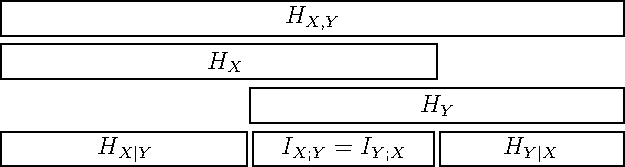
\includegraphics[width=0.7\linewidth]{mutualinf}\pause
    \end{center}
  \item Shannon defined the \textit{capacity} of a noisy channel as
    \begin{align*}
      C = \max_{\Prob{X}} I_{X;Y}
    \end{align*}
  \item That is, you choose the probability distribution of the
    message to maximise the information gain\pause
  \end{itemize}
\end{PauseHighLight}

\end{slide}

%%%%%%%%%%%%%%%%%%%%%%% Next Slide %%%%%%%%%%%%%%%%%%%%%%%

\begin{slide}
\section{Independent Noise}

\begin{rightImage}[0.2]{oneBitEntropy}
\begin{PauseHighLight}
  \begin{itemize}
  \item The simplest model of a noisy channel is a binary channel
    where each symbol is corrupted independently with a probability $f$
    \begin{align*}
      \Prob{X=1|Y=0}=\Prob{X=0|Y=1}=f\pause
    \end{align*}
  \item An elementary calculations shows that
    \begin{align*}
      H_{X_i|Y_i} = - (1-f)\,\log(1-f) - f\,\log(f) = H(f)\pause
    \end{align*}
  \item For a message of length $n$, $H_{X|Y} = n\,H(f)$\pause
  \end{itemize}
\end{PauseHighLight}
\end{rightImage}
  
\end{slide}

%%%%%%%%%%%%%%%%%%%%%%% Next Slide %%%%%%%%%%%%%%%%%%%%%%%

\begin{slide}
\section[-1]{Error Correcting Codes}
  
\begin{PauseHighLight}
  \begin{itemize}
  \item To reduce the chance of misinterpreting a message we need to
    build an error correcting code\pause
  \item We can do this dividing the space of binary messages into a
    set of Hamming balls
    \begin{center}
       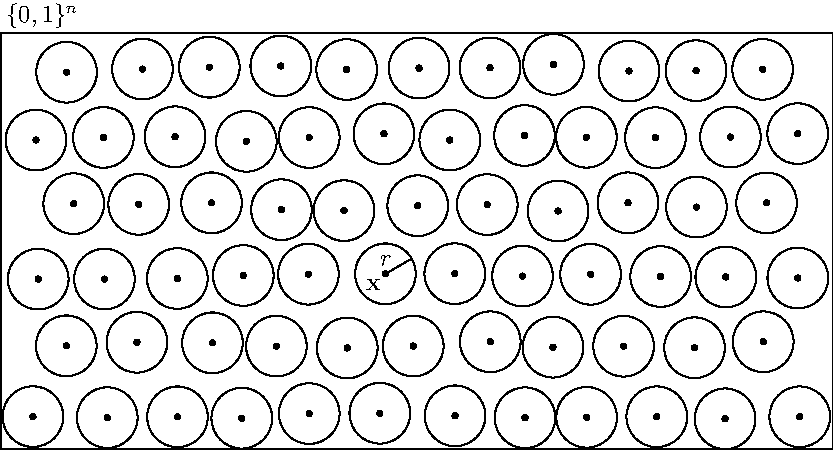
\includegraphics[width=0.5\linewidth]{shannonBound}\pause
    \end{center}
  \item A Hamming ball $B(\bm{x}, r)$ is the set of strings that
    differ from $n$-dimensional binary string, $\bm{x}$, by at most
    $r$ digits\pause
  \end{itemize}
\end{PauseHighLight}

\end{slide}

%%%%%%%%%%%%%%%%%%%%%%% Next Slide %%%%%%%%%%%%%%%%%%%%%%%

\begin{slide}
\section[-1]{Volume of Coding Space}

\begin{PauseHighLight}
  \begin{itemize}
  \item The expected number of errors in a string of length $n$ given
    an error rate of $f$ is $n\,f$\pause
  \item For sufficiently large $n$ we would expect all errors are
    smaller than $(f+\epsilon)\,n$ (for $\epsilon>0$)\pause
  \item If we make the radius of the Hamming ball $r=(f+\epsilon)\,n$
    ($\epsilon>0$) then we would expect no error for sufficiently large
    $n$\pause
  \item An upper bound on the number of code words we can send in a
    string of length $n$ is
    \begin{align*}
      \frac{2^n}{|B(\bm{x}_i, r)|} = c\,\sqrt{n} \, 2^{I_{X;Y}}\pause
    \end{align*}
  \end{itemize}
\end{PauseHighLight}
\end{slide}

%%%%%%%%%%%%%%%%%%%%%%% Next Slide %%%%%%%%%%%%%%%%%%%%%%%

\begin{slide}
\section[-1]{Lower Bounds}
  
\begin{PauseHighLight}
  \begin{itemize}
  \item Shannon also showed that choosing  $2^{I_{X;Y}}$ random
    strings of length $n$ the Hamming distance beween balls would be
    at least $f$ with high probability\pause
  \item This means that we can send information at rate of
    $I_{X;Y}$\pause
  \item The maximum rate is given by the channel capacity $\max I_{X;Y}$\pause
  \item If $f=0.1$ then $C=I_{X;Y} = 0.469 \bits$ so we need codes of
    just over twice as long to communicate accurately over a noisy
    channel with a 10\% corruption rate\pause
  \item Unfortunately, we can't efficiently decode random code
    positions, so although we know Shannon's bound is achievable we
    don't have practical codes that do this\pause
  \end{itemize}
\end{PauseHighLight}

\end{slide}

%%%%%%%%%%%%%%%%%%%%%%% Next Slide %%%%%%%%%%%%%%%%%%%%%%%

\begin{slide}
\section{Using Mutual Information}

\begin{PauseHighLight}
  \begin{itemize}
  \item Mutual information is used quite often in machine
    learning\pause
    \begin{itemize}
    \item Wikipedia mentions 14 applications\pause
    \end{itemize}
  \item Suppose we want to align two sets of images through some non-linear
    transformations\pause
  \item One way of doing this is to choose the non-linear
    transformations that maximise the mutual information (or
    normalised mutual information) between the two sets of images\pause
  \end{itemize}
\end{PauseHighLight}

\end{slide}


%%%%%%%%%%%%%%%%%%%%%%% Next Slide %%%%%%%%%%%%%%%%%%%%%%%
\Outline % KL-Divergence
%%%%%%%%%%%%%%%%%%%%%%% Next Slide %%%%%%%%%%%%%%%%%%%%%%%

\begin{slide}
\section[-2]{KL-Divergence}

\begin{PauseHighLight}
  \begin{itemize}
  \item We have met the Kullback-Leibler  divergence
    \begin{align*}
      \KL{p}{q} = \av[X\sim p(X)]{\logg{\frac{p(X)}{q(X)}}} \\
      = -\av[X\sim p(X)]{\logg{q(X)}} - H_X\pause
    \end{align*}
  \item Recall $-\logg{q(X=x)}$ is the length of code need to send a
    message $x$ with a probability $q(X=x)$\pause
  \item  Thus $-\av[X\sim p(X)]{\logg{q(X)}}$ is the expected length of
    message needed to code $X\sim p(X)$ using the optimal code for the
    distribution $q(X)$ that than $p(X)$\pause
  \item $\KL{p}{q}$ is also known as the \emph{relative entropy}
    and measures the expected extra length in coding $X\sim p(X)$ if
    we use the wrong distribution $q(X)$\pause
  \end{itemize}
\end{PauseHighLight}

\end{slide}

%%%%%%%%%%%%%%%%%%%%%%% Next Slide %%%%%%%%%%%%%%%%%%%%%%%

\begin{slide}
\section{Variational Approximation}

\begin{PauseHighLight}
  \begin{itemize}
  \item Recall we use MCMC in Bayesian inference because the posterior
    distribution is too complicated to write down in closed form\pause
  \item In the variational approximation we approximate the posterior
    distribution by a simpler (typically factored distribution), e.g.
    \begin{align*}
      f(\bm{\theta}\mid\data) \approx g(\bm{\theta}\mid\bm{\phi}) = \prod_i
      g(\theta_i\mid\phi_i)\pause
    \end{align*}
  \item The standard method for solving this is to maximise the
    \emph{variational free energy}
    \begin{align*}
      \Phi(\bm{\phi}) = -\int g(\bm{\theta}\mid\bm{\phi})
      \logg{\frac{g(\bm{\theta}\mid\bm{\phi})}{f(\bm{\theta}, \data)}} \,
      \dd \bm{\theta}\pause
    \end{align*}
  \end{itemize}
\end{PauseHighLight}

\end{slide}

%%%%%%%%%%%%%%%%%%%%%%% Next Slide %%%%%%%%%%%%%%%%%%%%%%%

\begin{slide}
\section{Evidence Lower Bound (ELBO)}

\begin{PauseHighLight}
  \begin{itemize}
  \item We can re-write the variational free energy as
    \begin{align*}
      \Phi(\bm{\phi}) &= -\int g(\bm{\theta}\mid\bm{\phi})
      \logg{\frac{g(\bm{\theta}\mid\bm{\phi})}{\bra{f(\bm{\theta},
                          \data)/f(\data)} \, f(\data)}} \,  \dd \bm{\theta}\pause
      \\
      &=  -\int g(\bm{\theta}\mid\bm{\phi}) \, \bra{
      \logg{\frac{g(\bm{\theta}\mid\bm{\phi})}{f(\bm{\theta}
                          \mid\data)} } - \logg{f(\data)} }\, \dd
        \bm{\theta}\pause
        \\
                        &= -\KL{g(\bm{\theta}\mid\bm{\phi})}{f(\bm{\theta}\mid \data)}
                           + \logg{f(\data)}\pause
    \end{align*}
    \item If we maximise $\Phi(\bm{\phi})$, we end up minimising the KL
      divergence between $g$ and $f$ so that $g\approx f$ and
      $\Phi(\bm{\phi})\approx \logg{f(\bm{D})}$\pause
    \item That is, we choose the parameters of our simple  factorised
      distribution so that it is close to the true posterior\pause
  \end{itemize}
\end{PauseHighLight}

\end{slide}

%%%%%%%%%%%%%%%%%%%%%%% Next Slide %%%%%%%%%%%%%%%%%%%%%%%

\begin{slide}
\section[-2]{Put Another Way}

\begin{PauseHighLight}
  \begin{itemize}
  \item We can rewrite the variational free energy as $\Phi(\bm{\phi})
    = L_q(\bm{\phi}) + H_q(\bm{\phi})$ where
    \begin{align*}
      L_q(\bm{\phi}) = \int g(\bm{\theta}\mid\bm{\phi}) \bra{
      \logg{\strut f(\data| \bm{\theta})} + \logg{f(\bm{\theta})} } \, \dd \bm{\phi}
    \end{align*}
    acts like an expected posterior term that is maximised when the
    data is well modelled (we put the probability density,
    $g(\bm{\theta}\mid\bm{\phi})$ where the $f(\bm{\theta}, \data)$ is
    large)\pause
  \item The second term is an entropy
    \begin{align*}
      H_q(\bm{\phi}) = - \int g(\bm{\theta}\mid\bm{\phi})
      \logg{\strut g(\bm{\theta}\mid\bm{\phi})} \dd \bm{\phi}
    \end{align*}
    That is, we maximise the uncertainty of the distribution $g(\bm{\theta}\mid\bm{\phi})$\pause
  \end{itemize}
\end{PauseHighLight}

\end{slide}


%%%%%%%%%%%%%%%%%%%%%%% Next Slide %%%%%%%%%%%%%%%%%%%%%%%

\begin{slide}
\section[-2]{Using Variational Methods}

\begin{PauseHighLight}
  \begin{itemize}
  \item Variational methods can be much faster than MCMC (although
    they tend to involve some iterations to minimise the variation
    free energy)\pause
  \item The can produce very good approximations, although this is not
    guaranteed (depends on the problem)\pause
  \item They can be extended (e.g. by minimising $\KL{g}{f}$
    rather than $\KL{f}{g}$---this is known as\textit{ belief
      propagation})\pause
  \item MCMC is less elegant, but is a controlled approximation (we get
    better results by increasing the number of iterations)\pause
  \item MCMC is slower, but on modern computers this isn't usually a
    problem\pause
  \end{itemize}
\end{PauseHighLight}

\end{slide}




%%%%%%%%%%%%%%%%%%%%%%% Next Slide %%%%%%%%%%%%%%%%%%%%%%%
\Outline % Minimum Description Length
%%%%%%%%%%%%%%%%%%%%%%% Next Slide %%%%%%%%%%%%%%%%%%%%%%%

\begin{slide}
\section[-1]{Compression and Model Selection}
  
\begin{PauseHighLight}
  \begin{itemize}
  \item Outside of the Bayesian framework it is difficult to do model
    selection\pause---most of ML isn't Bayesian\pauseb
  \item When is it better to accept a more complex model for a better
    fit and when are we just over-fitting?\pause
  \item Usually we answer this using a validation set, but this is not
    always possible\pause
  \item One principled approach is to use the model that allows us to
    maximally compress the data\pause
  \item If we are compressing the data then we are capturing features
    of the data\pause
  \end{itemize}
\end{PauseHighLight}

\end{slide}

%%%%%%%%%%%%%%%%%%%%%%% Next Slide %%%%%%%%%%%%%%%%%%%%%%%

\begin{slide}
\section{Alice and Bob}
  
\begin{PauseHighLight}
  \begin{itemize}
  \item Suppose Alice has data
    $\data=\{(\bm{x}_i,y_i) \mid i=1,2,\ldots,m\}$ while Bob  has only  the
    feature vectors $\{\bm{x}_i \mid i=1,2,\ldots,m\}$\pause
  \item Alice wants to communicate $y_i$ to Bob as efficiently as
    possible\pause
  \item We suppose Alice \& Bob have available a model
    $\hat{f}(\bm{x}|\bm{\theta})$\pause
  \item Rather than sending the complete list $\{y_i \mid
      i=1,2,\ldots,m\}$ Alice can send Bob the parameter
      $\bm{\theta}$ and the errors
      \begin{align*}
        \delta_i = y_i - \hat{f}(\bm{x}_i|\bm{\theta})\pause
      \end{align*}
    \item Assuming the $\delta_i$'s have a distribution $p_\delta$
      then the cost of communicating an error to accuracy $\Delta$ is
      $-\logg{p_\delta(\delta_i)\times\Delta}$\pause
  \end{itemize}
\end{PauseHighLight}

\end{slide}

%%%%%%%%%%%%%%%%%%%%%%% Next Slide %%%%%%%%%%%%%%%%%%%%%%%

\begin{slide}
\section{Description Length}

\begin{PauseHighLight}
  \begin{itemize}
  \item The \emph{description length} for $\{y_i \mid i=1,2,\ldots,m\}$ is
    then the cost of transmitting $\bm{\theta}$ plus the cost of
    transmitting the errors
    \begin{align*}
      L = \sum_{k=1}^n \ell(\theta_k) - \sum_{i=1}^m \bra{\logg{\strut p_\delta\!\left(y_i -
      \hat{f}(\bm{x}_i|\bm{\theta})\right)} + \logg{\Delta}}
    \end{align*}
    where $\ell(\theta_k) $ is the number of bits need to communicate
    $\theta_k$ (we get to choose the accuracy if is worth encoding the
    parameters)\pause
  \item To select between models we choose the model with the
    \emph{minimum description length}\pause
  \item Note that the accuracy $\Delta$ will lead to the same cost,
    $-m\,\logg{\Delta}$, for all models so doesn't affect which model is selected\pause
  \end{itemize}
\end{PauseHighLight}

\end{slide}

%%%%%%%%%%%%%%%%%%%%%%% Next Slide %%%%%%%%%%%%%%%%%%%%%%%

\begin{slide}
\section[-1]{Minimum Description Length (MDL) Method}

\begin{PauseHighLight}
  \begin{itemize}
  \item The minimum description length method can be a powerful way of
    choosing between models\pause
  \item Often it is the only principled method available\pause
  \item It allows you to trade model accuracy against model
    complexity\pause
  \item It can be fiddly as we need to determine the accuracy to which
    we should store the parameters of our model\pause
  \item This isn't something we usually think about, but often we can
    get very good models  even when we truncate the parameters to low
    precision\pause
  \end{itemize}
\end{PauseHighLight}

\end{slide}



%%%%%%%%%%%%%%%%%%%%%%% Next Slide %%%%%%%%%%%%%%%%%%%%%%%
\Outline % VAEs
%%%%%%%%%%%%%%%%%%%%%%% Next Slide %%%%%%%%%%%%%%%%%%%%%%%

\begin{slide}
\section[-2]{Variational Auto-Encoders VAE}

\pb
\pause\pauselevel{=1}

\begin{center}
  \multipdf[width=\linewidth]{vae}\pause
\end{center}
\begin{align*}
    \mathcal{L} =
  \av[\bm{x}\sim\mathcal{D}]{
  \KL{q_{\bm{\theta}}(\bm{z}|\bm{x})}{\mathcal{N}(\bm{0},\mat{I})}
  - \logg{p_{\bm{\theta}}(\bm{x}|\bm{z}(\bm{x}))}}\pause
\end{align*}
\end{slide}


%%%%%%%%%%%%%%%%%%%%%%% Next Slide %%%%%%%%%%%%%%%%%%%%%%%

\begin{slide}
\section[-2]{Latent Space}

\pb\pause\pauselevel{=1}
\begin{center}
  \multipdf[width=0.6\linewidth]{latentSpace}\pause
\end{center}
\begin{align*}
  \KL{q_{\bm{\theta}}(\bm{z}|\bm{x})}{\mathcal{N}(\bm{0},\mat{I})}\pauseb
\end{align*}
\end{slide}

%%%%%%%%%%%%%%%%%%%%%%% Next Slide %%%%%%%%%%%%%%%%%%%%%%%

\begin{slide}
\section[-2]{Understanding the Loss Function}

\begin{PauseHighLight}
  \begin{itemize}\squeeze
  \item The original paper derived the loss function as a variational
    approximation to maximising some posterior\pause
  \item This is difficult to understand (at least, for me)\pause
  \item It has a very natural explanation in terms of minimum
    description length\pause
  \item Alice wants to communicate the images to Bob\pause
  \item Alice uses the encoder to derive a (latent) code
    $q(\bm{z}|\bm{x})$ which she communicates to Bob\pause
  \item She also communicates the errors $\bm{\delta}=\bm{x}-\bar{\bm{x}}$\pause
  \item Bob uses the decoder to decode $q(\bm{z}|\bm{x})$ and
    $\bm{\delta}$ to repair the images\pause
  \end{itemize}
\end{PauseHighLight}


\end{slide}

%%%%%%%%%%%%%%%%%%%%%%% Next Slide %%%%%%%%%%%%%%%%%%%%%%%

\begin{slide}
\section[-1]{Description Length}

\begin{PauseHighLight}
  \begin{itemize}
  \item The loss
    \begin{align*}
      \mathcal{L} =
      \av[\bm{x}\sim\mathcal{D}]{
      \KL{q_{\bm{\theta}}(\bm{z}|\bm{x})}{\mathcal{N}(\bm{0},\mat{I})}
      - \logg{p_{\bm{\theta}}(\bm{x}|\bm{z}(\bm{x}))}}\pause
    \end{align*}
    can be interpreted as
    \begin{itemize}
    \item The cost of communicating the code
      $\KL{q_{\bm{\theta}}(\bm{z}|\bm{x})}{\mathcal{N}(\bm{0},\mat{I})}$\pause
    \item Plus the cost to send the repair $ \logg{p_{\bm{\theta}}(\bm{x}|\bm{z}(\bm{x}))}$\pause
    \end{itemize}
  \item We minimise the loss function\pause{} equivalent to MDL\pauseb
  \item What is really clever is that we can choose the accuracy of
    the code we send $q_{\bm{\theta}}(\bm{z}|\bm{x})$ to minimise the
    over-all cost\pause
  \end{itemize}
\end{PauseHighLight}

\end{slide}


%%%%%%%%%%%%%%%%%%%%%%% Next Slide %%%%%%%%%%%%%%%%%%%%%%%

\begin{slide}
\section{Conclusions}

\begin{PauseHighLight}
  \begin{itemize}
  \item Information theory has regularly been used in machine
    learning\pause
  \item It requires some understanding and care to do it
    properly\pause
  \item The KL-divergence (or relative entropy) is often used to make
    two probability distribution more alike\pause
  \item The minimum description length is a powerful principle for
    model selection\pause
  \item Variational Auto-Encoders have a very natural interpretation
    in terms of minimising a description length\pause
  \end{itemize}
\end{PauseHighLight}


\end{slide}


%%% Local Variables:
%%% TeX-master: "lectures"
%%% End:
